\documentclass[conference]{IEEEtran}
\IEEEoverridecommandlockouts
% The preceding line is only needed to identify funding in the first footnote. If that is unneeded, please comment it out.
\usepackage{cite}
\usepackage{amsmath,amssymb,amsfonts}
\usepackage{algorithmic}
\usepackage{graphicx}
\usepackage{textcomp}
\usepackage{xcolor}
\def\BibTeX{{\rm B\kern-.05em{\sc i\kern-.025em b}\kern-.08em
    T\kern-.1667em\lower.7ex\hbox{E}\kern-.125emX}}
\begin{document}

\title{Autonomous Driving for the Texas Instruments Cup}

\author{\IEEEauthorblockN{Mohammed Fareed}
\IEEEauthorblockA{\textit{Kate Gleason College of Engineering} \\
\textit{Department of Computer Engineering}\\
Rochester, NY \\
mff9108@rit.edu}
\and
\IEEEauthorblockN{Trent Wesley}
\IEEEauthorblockA{\textit{Kate Gleason College of Engineering} \\
\textit{Department of Computer Engineering}\\
Rochester, NY \\
taw8452@rit.edu}
}

\maketitle

\begin{abstract}
Autonomous driving is progressing and becoming more prevelant in society as time goes by. A robust autonomous driving system offers the potential for a future where driving safety and efficiciency are dramatically increased. The Rochester Institute of Technology Texas Instruments Car Cup required the application of various autonomous driving techniques and algorithms to race. The objective of this project was to program a miniature battery powered car to autonomously race around a track. The car was controlled by an MSP432 microcontroller board used the input from a linescan camera to control its servo and motors for steering and speed control. This paper documents the theory, code development, and the challenges to race in the fall 2023 Texas Instruments Cup.
\end{abstract}

\section{Introduction}
Every semester, Rochester Institute of Technology (RIT) hosts a Texas Instruments (TI) autonomous car race. This challenges computer engineering students to use their skills and knowledge regarding microcontrollers, motor control, control systems, and problem solving. Given that there is an average of 6 million car accidents in the US every year, education and experience with autonomous driving can help shape a world where driving is much safer \cite{accidentStats}.

The cars utilized had various components with different functions. The cars included two motors (one for each back wheel), a servo for steering, and MSP432 microcontroller board for control, a linescan camera, and OLED display, and a 7.2V battery pack. A picture of the car used is shown in Figure \ref{fig:car}.

\begin{figure}[htbp]
	\centerline{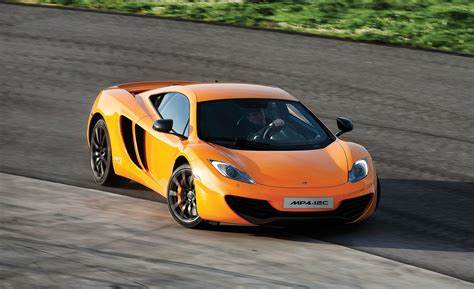
\includegraphics[width=0.45\textwidth]{images/car.jpg}}
	\caption{Car.}
	\label{fig:car}
\end{figure}

The racetrack developed for the TI Cup tested various aspects of autonomous racing. It combined performance on straight aways, turns, intersections, hills, and wobbles. To perform well on the track, a car would need to be able to handle all of these conditions. A picture of the track is shwon in Figure \ref{fig:track}.

\begin{figure}[htbp]
	\centerline{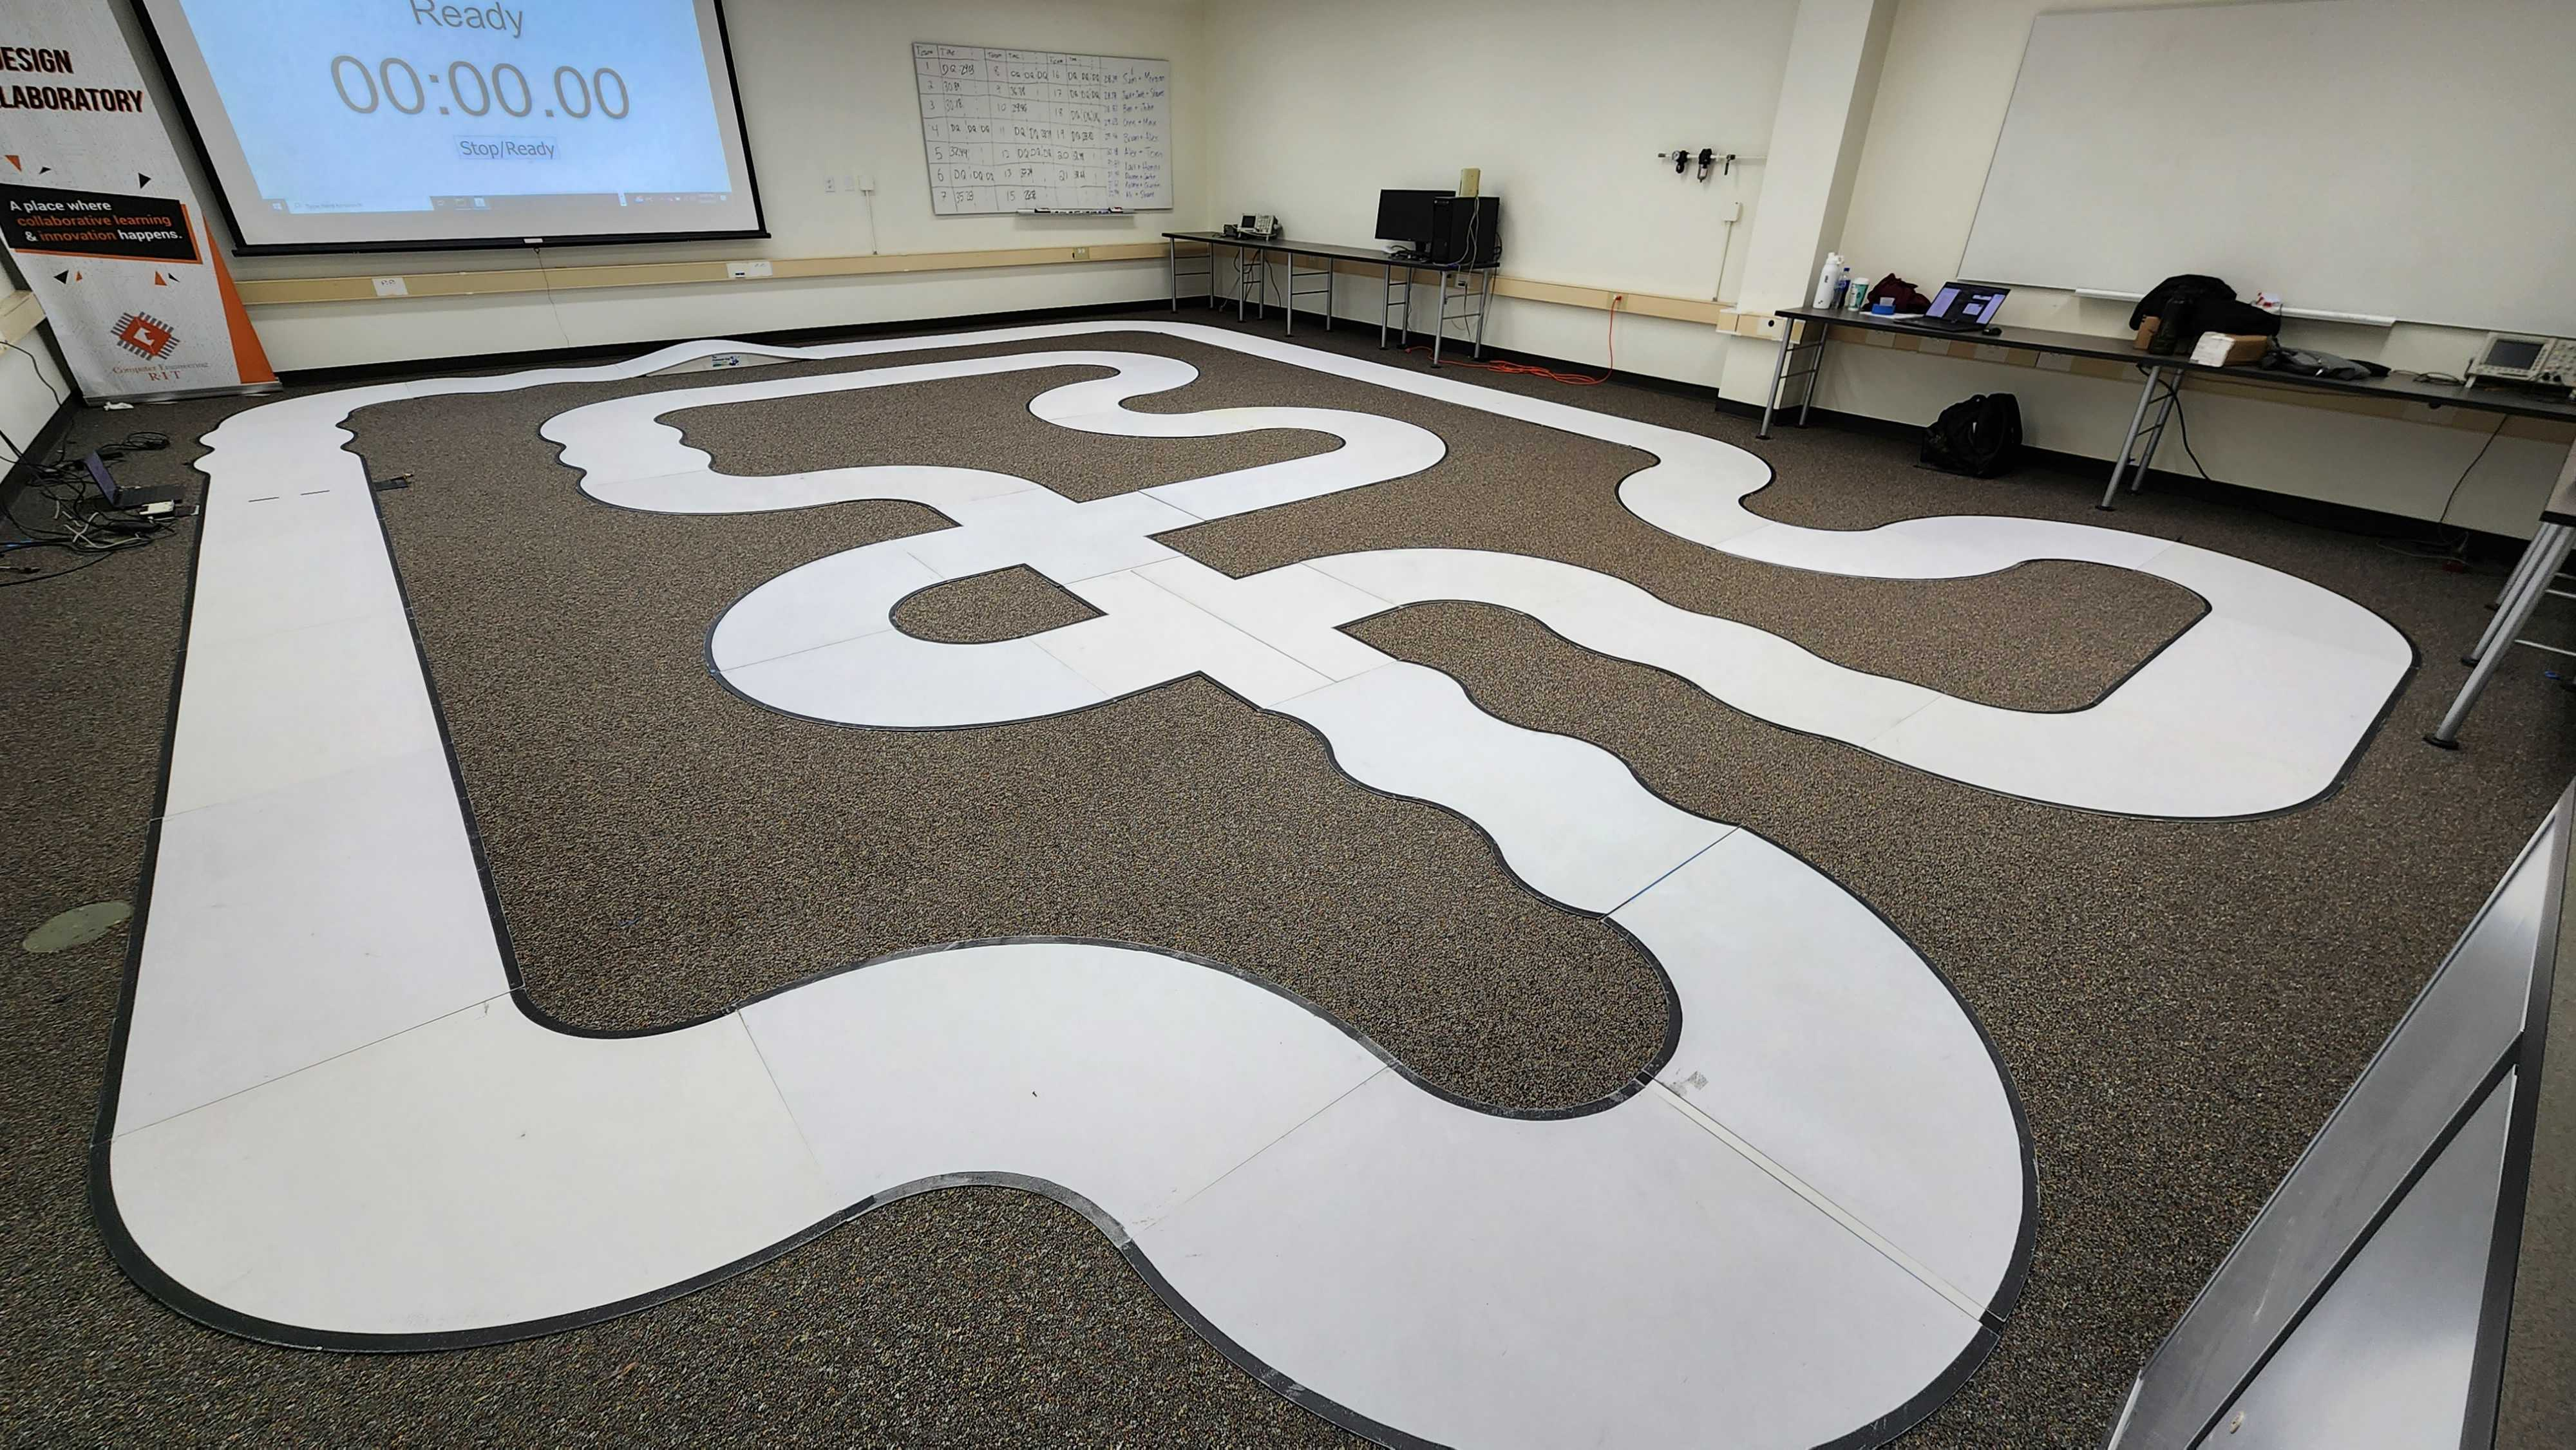
\includegraphics[width=0.45\textwidth]{images/track.jpg}}
	\caption{Racetrack for TI Cup.}
	\label{fig:track}
\end{figure}

The rest of this paper is organized as follows. Section 2 discusses background information regarding the TI Cup, some general theory applied, some of the MSP432 modules used, and some of the hardware used. Section 3 covers the proposed method and specific implementations for the project. Section 4 presents the results of the race and performance of the car. Section 5 gives a conclusion of the project. Section 6 gives the authors' acknowledgements. Section 7 lists the references used for this paper.

\section{Background}

\subsection{RIT TI Car Cup}

The RIT TI Car Cup is hosted every fall and spring semester. Each team has three attempts to complete one lap on the track as fast as possible. The first time a lap is completed is the final time. If a team doesn't finish in three attempts, they are disqualified. For an lap to be considered successful, the car must finish in under 60 seconds and have at least two wheels on the track at all times. Race results were recorded by a laser timer for accuracy.

\subsection{Materials}

The car has many components and generates a price from them. Reference \cite{carCup2022} was observed to create the bill of materials shown in Table \ref{table:billOfMaterials}. 

\begin{table}[htbp]
\caption{Bill of Materials}
\begin{center}
\begin{tabular}{|c|c|c|}
\hline
Part & Qty & Cost (USD) \\
\hline
Parallax TSL-1401 Line Scan Camera & 1 & \$80.00 \\
\hline
Servo Steering Arms & 1 & \$17.99 \\
\hline
Motor Driver - RB-WAV-77 & 1 & \$28.9 \\
\hline
Car Chassis Kit - ROB0170 & 1 & \$98.75 \\
\hline
Brushed DC Motor Kit - KIT0167 & 1 & \$25.00 \\
\hline
UCTRONICS Module 12864 SSD1306 OLED & 1 & \$6.99 \\
\hline
Bluetooth Module HM-10 & 1 & \$10.99 \\
\hline
Tenergy 7.2V High Capacity 6-Cell Battery Pack & 1 & \$39.99 \\
\hline
Sourcingpower Universal RC Battery Charger & 1 & \$19.99 \\
\hline
Fielect 5Pcs F-F 6Pin Jumper Wire Ribbon Cable & 1 & \$6.69 \\
\hline
5pcs Tamiya Male Power Connector Cable & 1 & \$8.68 \\
\hline
Zip Ties & 1 & \$18.99 \\
\hline
\textbf{Total} & & \textbf{\$363.05} \\
\hline
\end{tabular}
\label{table:billOfMaterials}
\end{center}
\end{table}

The bill of materials gives information about parts, quantity, and cost in USD. As shown in Table \ref{table:billOfMaterials}, a total of approximately \$363.05 would need to be spent to construct a similar car.

\subsection{Camera}

\subsection{Motors}

\subsection{PID theory}

\subsection{Timers and Interrupts}

\subsection{Analog to Digital Converter}

\section{Proposed Method}

\subsection{Camera Vision and Filtering}

The linescan camera's output is an array of 128 integers representing the brightness it sees. The linescan camera used had a maximum value of $2^{14}$-1 (16383), and would tend to saturate at that value pretty easily. This phenomenon was utilized to filter out the carpet from what was the track. If an array element was less than 16381, it wouldn't be considered as part of the track and would be treated as 0. Otherwise, the element would be treated as a 1. This creates a binary representation of track versus carpet. Figure \ref{fig:linescan} shows a plot characterizing the typical behavior of the linescan camera.

\begin{figure}[htbp]
	\centerline{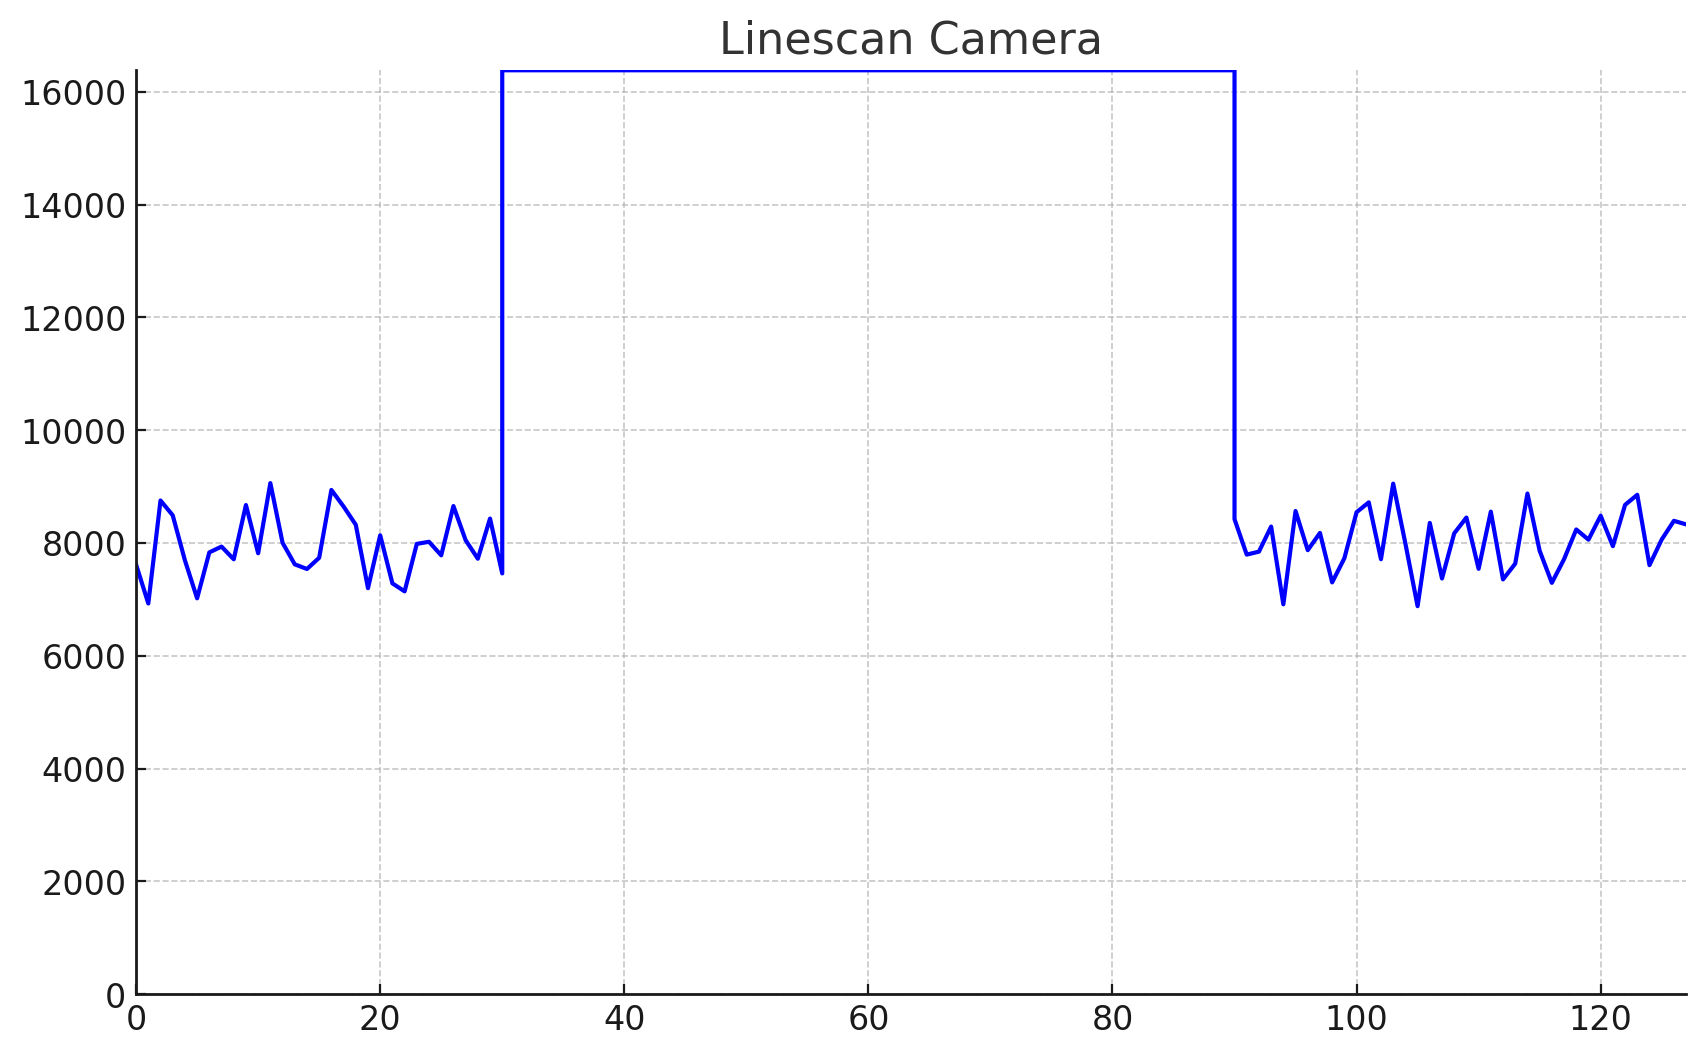
\includegraphics[width=0.45\textwidth]{images/linescan.png}}
	\caption{Unfiltered Linescan Output.}
	\label{fig:linescan}
\end{figure}

In Figure \ref{fig:linescan}, the saturated component is where the linescan camera sees the bright white track along the 128 elements of the array. The rest is the where the camera sees the darker carpet beside the track. As stated, this output was filtered into a binary representation of where there is and isn't track. This output is modeled by Figure \ref{fig:linescanFiltered}.

\begin{figure}[htbp]
	\centerline{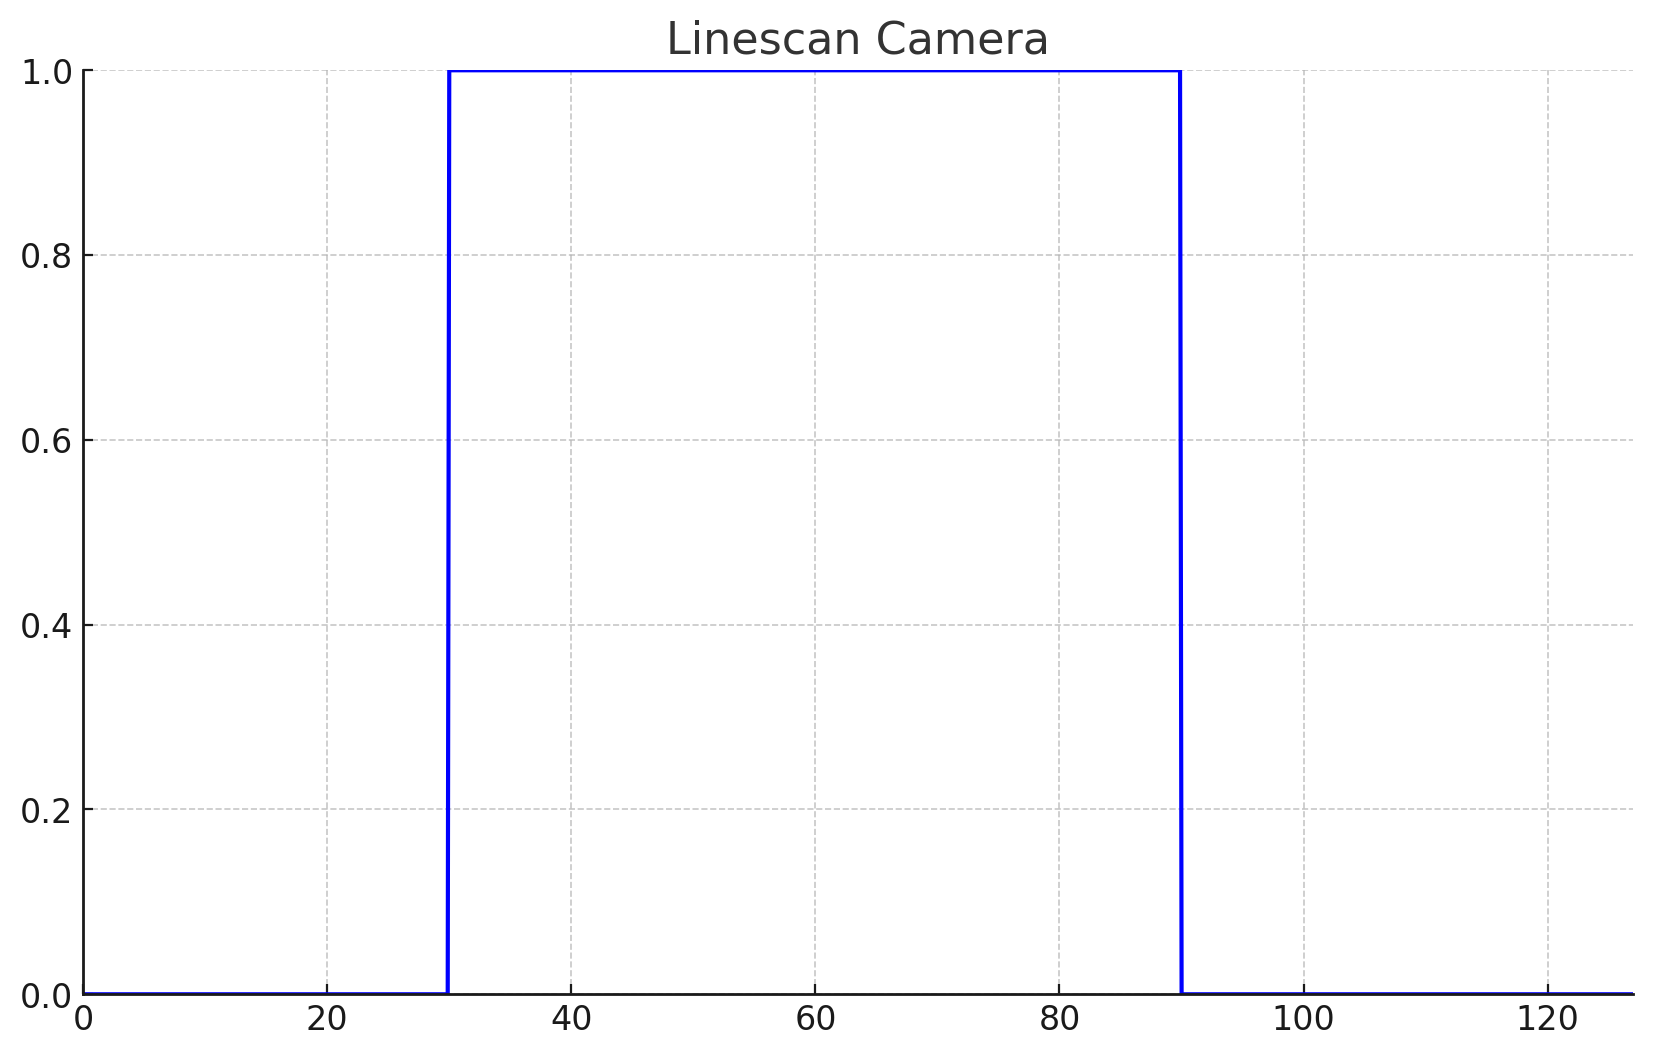
\includegraphics[width=0.45\textwidth]{images/linescanFiltered.png}}
	\caption{Filtered Linescan Output.}
	\label{fig:linescanFiltered}
\end{figure}

This filtered output is simpler and unbiased by the values unassociated with the track. Using the binary output, a weighted average was calculated to find where the center of the track is. The calculation is shown in Equation \ref{eq:midpoint}.

\begin{equation}
	\text{midpoint} = \frac{\sum_{i=0}^{127} i*x_i}{\sum_{i=0}^{127} x_i}\label{eq:midpoint}
\end{equation}

In Equation \ref{eq:midpoint}, $i$ represents the index in the array and $x_i$ represents the binary value at the index in the array. The resulting midpoint can the be used to determine the position of the middle of the track and steer towards it.

\subsection{Carpet Detection}

Carpet detection is important for preventing damage from hitting a wall when the car would drive off the track. The program logic created to detect whether the car has left the track is very simple. Every element of the raw output array from the linescan camera was added up. This sum was compared to a brightness threshold calibrated through trial and error. If the sum was less that the threshold, the car would stop the DC motors and therefore stop the car from moving.

\subsection{PID Implementation}

PID was utilized for steering with a servo to be able to handle turns and reduce oscillations on straight paths. Error is an essential variable for PID to function. For this project, error was the calculated as shown in Equation \ref{eq:error}.

\begin{equation}
	\text{error} = \text{midpoint} - 64.5 \label{eq:error}
\end{equation}

On a scale from 0 to 127 (indices of linescan camera output), the midpoint would normally be 63.5. In this case, it was 64.5 to adjust for the offset of the camera. This calculated error was then used for PID control. The overall equation for to control the servo with PID is shown in Equation \ref{eq:PID}.

\begin{equation}
	ServoPWM = K_p*\text{error1} + K_i*\frac{\text{error} + \text{error2} + \text{error3}}{3} 
	+ K_d*(\text{error1} - 2*\text{error2} + \text{error3}) \label{eq:PID}
\end{equation}

In this Equation \ref{eq:PID}, error1 refers to the most recent error, error2 refers to the error before error1, and error3 refers to the error before error2. This error history allows the PID algorithm to respond in a more optimal way than if it only had access to the the most recent error. 

This calculation alone is not sufficient since a servo PWM outside of the range 0.05 to 0.1 could break the car. For this reason, code was added which would set the servo's PWM to 0.05 if the calculated value was less than 0.05. Additionally, the code would set the servo's PWM to 0.1 if the calculated value was greater than 0.1.

\subsection{Variable Speed}

Variable speed was implemented so that the car would slow down when turning and speed up when going straight. Specifically, this was implemented with an equation relating the absolute value of servo's PWM input (0.05 to 0.1 duty cycle) minus its middle position (0.075 duty cycle). The more the servo position varied from the center, the slower the car was programmed to go. This is shown in Equation \ref{eq:speed}.

\begin{equation}
	\text{MotorPWM} = -18*|\text{ServoPWM} - 0.075| + 0.434 \label{eq:speed}
\end{equation}

If the motor PWM calculated is less than 0.36, it was set to 0.36 by the code to ensure it was maintaining a decently fast speed.

\section{Results}

\subsection{Race Results}


\section*{Acknowledgments}

\begin{thebibliography}{00}
\bibitem{accidentStats} “Car Accident Statistics in the U.S. | Driver Knowledge,” DriverKnowledge, 2019. https://www.driverknowledge.com/car-accident-statistics/
\bibitem{carCup2022} K. Jacowleff and M. Teichman, “Texas Instruments Autonomous Car Cup Project Fall 2022,” 2022.
\end{thebibliography}

\end{document}
